\chapter{Background}
\label{chap:background}

\section{Desiderata}

In this section, we review important desiderata for uncertainty estimation. We provide a summary of these desiderata in Tab.~\ref{tab:overview_desiderata}.

\begin{table*}[ht]
    \begin{center}
    \resizebox{1.\textwidth}{!}{%
    \begin{tabular}{ccc}
    \toprule
    \textbf{Bayesian distributions} & \textbf{Uncertainty types} & \textbf{Practical requirements} \\
    \midrule
    \midrule
    $\prior(\bm{\phi} \condition \data)$ where $\bm{\phi}$ are model weights &  Aleatoric uncertainty & Efficiency: Data \& Time \\
    $\prior(\bm{a} \condition \data, \x)$ where $\bm{a}$ are values of the activations &  Epistemic uncertainty & Flexibility: Architecture \& Optimization \\
    $\prior(\bm{\theta} \condition \data, \x)$ where $\bm{\theta}$ are parameters of the target distribution &  Predictive uncertainty & Robustness: Natural \& Adversarial \\
    \bottomrule
    \end{tabular}%
    }
    \end{center}
    \caption{Overview of desiderata for models for uncertainty estimation}
    \label{tab:overview_desiderata}
\end{table*}

\subsection{Bayes Formula} We recall the Bayes formula since it is a core concept in many uncertainty estimation approaches.
We define the distribution $\prob(\y \condition \bm{\theta})$ over the target variable $\y \in \real$ given the parameter $\bm{\theta}$.
Given a dataset $\data=\{\y^{(1)}, ..., \y^{(\ndata)}\}$, the Bayes formula is:
\begin{equation}
    \prior(\bm{\theta} \condition \data) = \frac{\prob(\data \condition \bm{\theta}) \times \prior(\bm{\theta})}{\prob(\data)}
\end{equation}
where $\prob(\data \condition \bm{\theta})$ is the \emph{likelihood}, $\prior(\bm{\theta})$ is the \emph{prior}, $\prior(\bm{\theta} \condition \data)$ is the \emph{posterior}, and $\prob(\data)$ is the \emph{evidence}.
Intuitively, the Bayesian formula updates the prior belief represented by $\prior(\bm{\theta})$ into the posterior belief represented by $\prior(\bm{\theta} \condition \data)$ after observing a dataset $\data$ \cite{bishop}.
The choice of prior is crucial. A common choice is to follow the \emph{principle of maximum entropy} \citep{maximum-entropy-principle} and enforce high entropy for the prior distribution which is usually considered less informative. However, note that many works studied different choices of priors \cite{jeffreys1946prior, silvestro2020prior}.
The evidence term $\prob(\data)$ corresponds to a normalization constant which can sometimes be ignored \cite{bishop}.

After observing a dataset $\data$, we can update the distribution over the target variable $\y$ in two ways.
A first option is to use a point-wise estimate of the target distribution parameter, i.e.:
\begin{equation}
    \prob(\y \condition \bm{\theta}^*)
\end{equation}
where $\bm{\theta}^*=\argmax\prior(\y \condition \bm{\theta})$ would be the maximum likelihood estimate, or $\bm{\theta}^*=\argmax\prior(\bm{\theta} \condition \data)$ would be the maximum a posteriori estimate.
A second option is to integrate over all possible values for the target distribution parameter, i.e.:
\begin{equation}
    \label{eq:posterior_predictive}
    \prob(\y \condition \data) = \int \prob(\y \condition \bm{\theta}) \prior(\bm{\theta} \condition \data) d\bm{\theta}
\end{equation}
where $\prob(\y \condition \data)$ is called the posterior predictive distribution. 
This second approach is often considered to be more Bayesian since it depends on the full posterior distribution $\prior(\bm{\theta} \condition \data)$.
However, it might be costly to compute the posterior distribution since it requires integration.

In supervised learning, the goal is to predict the value of a target output variable $\y$ given an input $\x$ after observing a dataset $\data=\{(\x^{(1)}, \y^{(1)}), ..., (\x^{(\ndata)}, \y^{(\ndata)})\}$.
In this case the posterior predictive requires to be adapted with three main options. The first option is:
\begin{equation}
    \prob(\y \condition \data, \x) = \int \prob(\y \condition \bm{\phi}, \x) \prior(\bm{\phi} \condition \data) d\bm{\phi}
\end{equation}
In this case, the parameter distribution $\prior(\bm{\phi} \condition \data)$ is not conditioned on the input $\x$ and only accounts for an uncertainty dependent on the dataset $\data$. Examples of such models are Bayesian neural networks which learn Bayesian distribution $\prior(\bm{\phi} \condition \data)$ where $\bm{\phi}$ denote the model weights \cite{bayesian-networks}.
The second option is:
\begin{equation}
    \prob(\y \condition \data, \x) = \int \prob(\y \condition \bm{a}) \prior(\bm{a} \condition \data, \x) d\bm{a}
\end{equation}
In this case, the parameter distribution $\prior(\bm{a} \condition \data, \x)$ is conditioned on the new input $\x$ and accounts for an uncertainty dependent on the input $\x$. Examples of such models are Bayesian neural networks which learn Bayesian distribution $\prior(\bm{a} \condition \data, \x)$ where $\bm{a}$ denote the values of the activations \cite{gp-uncertainty-activation,natural-parameter-network}.
Alternatively, the third option is:
\begin{equation}
    \prob(\y \condition \data, \x) = \int \prob(\y \condition \bm{\theta}) \prior(\bm{\theta} \condition \data, \x) d\bm{\theta}
\end{equation}
In this case, the parameter distribution $\prior(\bm{\theta} \condition \data, \x)$ is conditioned on the new input $\x$ and also accounts for an uncertainty dependent on the input $\x$. Examples of such models are the Bayesian neural networks proposed in this thesis \cite{charpentier2020,natpn, graph-postnet,charpentier2022uncertainty-rl,uceloss} which learn Bayesian distributions $\prior(\bm{\theta} \condition \data, \x)$ where $\bm{\theta}$ denote the parameters of the distribution over the target labels $\y$. In this thesis, we focus on learning  Bayesian distributions on the (generally) low dimensional target parameters $\bm{\theta}$ in contrast to the (generally) high dimensional activation $\bm{a}$ or weights  $\bm{\theta}$ which can advantageously allows to reduce the approximation complexity.

\subsection{Aleatoric, Epistemic \& Predictive Uncertainty}

The Equation~\ref{eq:posterior_predictive} involves three types of distribution (i.e. $\prob(\y \condition \bm{\theta})$, $\prior(\bm{\theta} \condition \data)$, and $\prob(\y \condition \data)$) which cover the three main sources of uncertainty (i.e. aleatoric, epistemic, and predictive).
In practice, each uncertainty type can be measured by computing the spread of its respective distribution with the (differential) entropy which represented its variability, i.e.:
\begin{align}
     u_\text{alea} = \entropy[\prob(\y \condition \bm{\theta})], \hspace{4mm}
     u_\text{epist} = \entropy[\prior(\bm{\theta} \condition \data)], \hspace{4mm}
     u_\text{pred} = \entropy[\prob(\y \condition \data)]
\end{align}
Apart from the entropy, other uncertainty metrics commonly use the variance of the distributions to indicate their variability. Finally, it is also to measure the variability of a distribution with their concentration parameters if they exist.

The \emph{aleatoric uncertainty} is sometimes also called data uncertainty, stochastic uncertainty or risk \cite{hullermeier2021aleatoric,knight1921, malini2018}. 
The aleatoric uncertainty is represented by the distribution $\prob(\y \condition \bm{\theta})$.
Beyond entropy computation, it can also be computed using max probability for classification \cite{malini2018}.
The aleatoric uncertainty should be high when \emph{the model does not know because of inherent noise in a given context} (e.g. noisy environment, noisy sensors, low computation resources, model mispecification) \cite{wenger2022posterior, hullermeier2021aleatoric}.
Given a specific context, the aleatoric uncertainty is \emph{irreducible} since additional observations cannot resolve the information loss due noisy measurements or misspecifications. 
However, aleatoric uncertainty can be reduced by using higher measurement resolution or improving the model specification. 

The \emph{epistemic uncertainty} is sometimes also called knowledge uncertainty, systematic uncertainty, knightian uncertainty \cite{hullermeier2021aleatoric,knight1921,malini2018}.
The epistemic uncertainty is represented by the distribution $\prior(\bm{\theta} \condition \data)$.
The epistemic uncertainty should be high when \emph{the model does not know because of a lack of observed data} in the dataset $\data$.
Hence, the epistemic uncertainty is \emph{reducible} since it should decrease when collecting additional data.

The \emph{predictive uncertainty} is sometimes also called total uncertainty \cite{hullermeier2021aleatoric,malini2018}.
The predictive uncertainty is represented by the distribution $\prob(\y \condition \data)$.
Intuitively, the predictive uncertainty aggregates the effect of the aleatoric and epistemic uncertainty by integrating jointly the distributions $\prob(\y \condition \bm{\theta})$ and $\prior(\bm{\theta} \condition \data)$. 

In this thesis, we focus on methods capable to estimates the three types of uncertainty types.

\subsection{Efficiency, Flexibility \& Robustness}

Uncertainty methods are also expected to have practical characteristics. 

First, an uncertainty method is expected to be \emph{efficient} at both training and testing time. 
A first aspect is \emph{time efficiency} meaning that the method should be fast with low computational overhead.
As second aspect is \emph{data efficiency} meaning that the method should require as few data as possible to train.

Second, an uncertainty method is expected to be \emph{flexible}.
A first aspect is \emph{architecture flexibility} meaning that the method should easily adapt to any architectures in order to easily adapt to different input types (e.g. tabular, images, graphs, and sequential data) and output types (e.g. classification and regression).
A second aspect is \emph{optimization flexibility} meaning that the method should easily adapt to different training schemes including end-to-end training or fine-tuning based on pretrained models.

Finally, an uncertainty method is expected to be \emph{robust}.
A first aspect is \emph{natural robustness} meaning that the method should be performant even if there is some natural drift in the data. Natural drifts could be due to time evolution or location variability \cite{wilds, neuhold201mapillary, shifts-dataset}.
A second aspect is \emph{adversarial robustness} meaning that the method should be performant even against adversarial perturbations which are specifically designed to fool the model. Adversarial perturbations can be viewed as the worst-case scenario for the model. Different methods to compute adversarial perturbations including white box attacks which do not have information about the model, black box attacks which have full access to the model information, and gray box which have partial information about the model \cite{han2020adversarial}.

In this thesis, we focus on proposing practical methods which are efficient in terms of data and time, flexible in terms of architecture and optimization schemes, and robust in terms of natural and adversarial perturbations.

\section{Models}

In this section, we review important family of models for uncertainty estimation. We provide a summary of these models in Fig.~\ref{fig:overview_methods}.

\begin{figure}[ht!]
    \centering
    \begin{subfigure}[t]{1. \columnwidth}
        \centering
        $\vcenter{\hbox{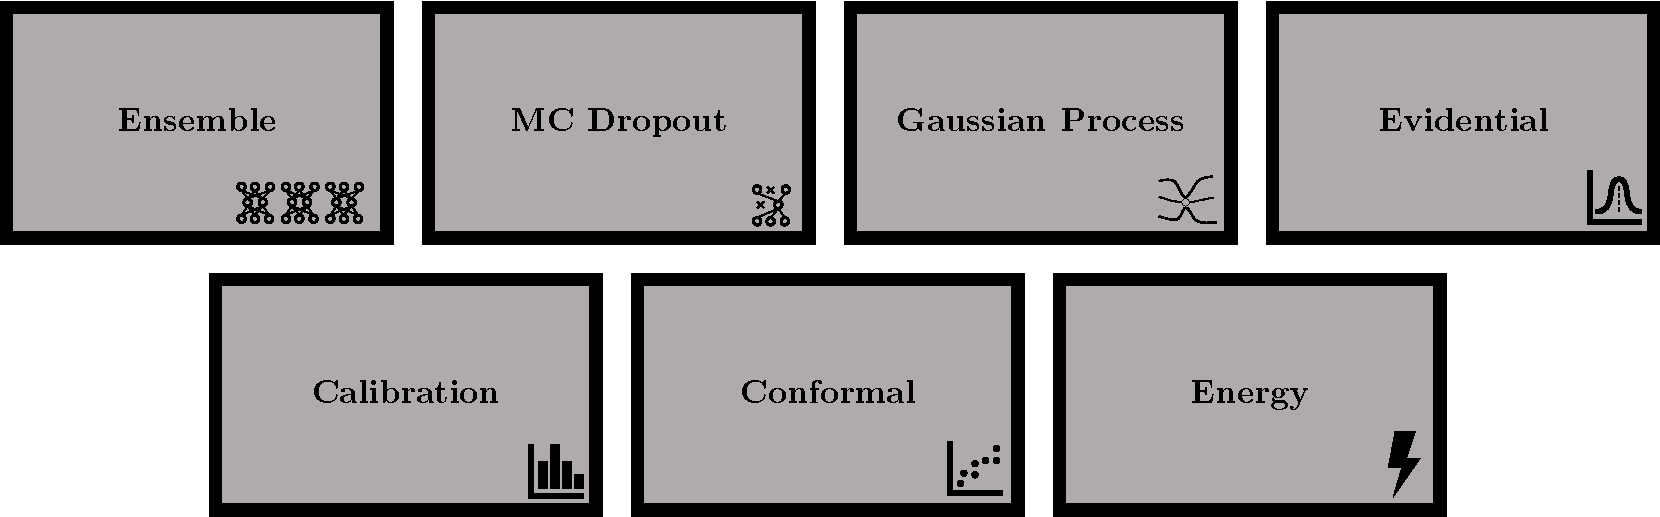
\includegraphics[width=0.9 \textwidth]{resources/overview_methods.pdf}}}$
    \end{subfigure}%
    \caption{Overview of the different families of methods for uncertainty estimation.}
    \label{fig:overview_methods}
	% \vspace{-.5cm}
\end{figure}

\subsection{Sampling-based models}

Sampling-based models estimate uncertainty by aggregating statistics (e.g. mean and variance) from different samples from a given distribution. The prediction generally follows a three steps process:
\textbf{(1)} we sample $K$ model weights $\bm{\phi}_k$ from a distribution over the weights $\prior(\bm{\phi} \condition \data)$, i.e. $\bm{\phi}_k \sim \prior(\bm{\phi} \condition \data)$. The type of the weight distribution $\prior(\bm{\phi} \condition \data)$ is a key design choice. E.g. ensemble proposes to train independent model weights \cite{ensembles}, MC dropout randomly drop weights with given dropout rate \cite{dropout}, and other Bayesian neural networks learn explicit distributions like Gaussian over the model weights \cite{bayesian-networks}. \textbf{(2)} We perform $K$ forward passes with the sampled model weights, i.e. $\bm{\theta}_k = f_{\bm{\phi}_k}(\x) \text{ for } k=1,..K$. This allows to implicitly sample the parameters $\bm{\theta}_k$ from the posterior distribution $\prior(\bm{\theta} \condition \data)$, i.e. $\bm{\theta}_k \sim \prior(\bm{\theta} \condition \data, \x)$. In this case, the parameters $\bm{\theta}_k$ can be the parameters of a categorical distribution for classification or the parameters of a Gaussian distribution for regression. \textbf{(3)} We aggregate the $\bm{\theta}_k$ parameters to form a point estimate $\bm{\theta}*$, e.g. $\bm{\theta}*=\frac{1}{K}\sum_k \bm{\theta}_k$. This allows to define the target distribution $\prob(\y \condition \bm{\theta}^*)$. These methods are flexible and allows to estimate all types of uncertainty while still being accurate. However, they often come to the cost of a higher computational cost due to the need of multiple forward passes.

\subsection{Sampling-free models}
Sampling-free models are capable of estimating uncertainty in a single forward pass. A first family of models explicitly parametrize the distribution $\prior(\bm{\theta} \condition \data, \x)$ with evidential distributions \citep{survey_evidential_uncertainty,robustness-uncertainty-dirichlet,max_gap_id_ood,uncertainty-generative-classifier,multifaceted_uncertainty,graph-postnet, lightweight-prob-net}. A second family aims at learning deep Gaussian processes on a learned latent space \citep{uncertainty-distance-awareness, due, duq, uceloss}. A third family aims at learning deep energy-based models \citep{ood_ebm, jem_ebm}. The GP and energy-based approaches might sometimes not be able to disentangle the different uncertainty types. Another family of models tries to recalibrate existing models by using calibration methods like temperature scaling \cite{calibration-network} or conformal predictions \cite{conformal-survey} which generally requires additional data to calibrate uncertainty estimates. Finally, a last family of models propagate uncertainty across layers \citep{natural-parameter-network, sampling-free-variance-propagation, feed-forward-propagation, lightweight-prob-net, probabilistic-backprop-scalable-bnn}. They model uncertainty at the weight and/or activation levels and are generally constrained to specific transformations.

\section{Experimental setup}

In this section, we present an exhaustive summary of the main metrics used to evaluate the quality of uncertainty estimation. 
It covers correct/wrong predictions detection, OOD \& dataset shifts detection, calibration, and sample efficiency.
We provide a collection of benchmarks which cover the different tasks in Tab.~\ref{tab:overview_evaluation}.

\begin{table*}[ht]
    \begin{center}
    \resizebox{1.\textwidth}{!}{%
    \begin{tabular}{ccc}
    \toprule
    \textbf{Evaluation setup} & \textbf{Existing Benchmarks} & \textbf{Practical reason}\\
    \midrule
    \midrule
    Correct/wrong pred. detection & \cite{robustness-uncertainty-dirichlet,Hendrycks2016, shifts-dataset, tran2022plex} & \emph{Trust} \\
    \midrule
    OOD detection & \cite{robustness-uncertainty-dirichlet,charpentier2022uncertainty-rl,yang2022openood, cao2020ood, kirchheim2022pytorch, Hendrycks2016,charpentier2022uncertainty-rl, tran2022plex} & \emph{Safety}\\
    \midrule
    Robustness to dataset shifts & \cite{robustness-uncertainty-dirichlet,wilds, neuhold201mapillary, shifts-dataset, benchmarking-corruptions, taori2020shift, dataset-shift, croce2021robustbench,charpentier2022uncertainty-rl, tran2022plex} & \emph{Maintenance} \\
    \midrule
    Uncertainty calibration & \cite{dataset-shift, chung2021uncertainty,nado2021uncertainty, tran2022plex} & \emph{Fairness}, \emph{Trust}\\
    \midrule
    Sample efficiency & \cite{charpentier2022uncertainty-rl,hsu2018continual, lin2021clear,antoniou2020fewshots,tran2022plex} & \emph{Maintenance}\\
    \bottomrule
    \end{tabular}%
    }
    \end{center}
    \caption{Overview of evaluation setups for uncertainty estimation}
    \label{tab:overview_evaluation}
\end{table*}

\subsection{Correct \& Wrong Predictions}

It is crucial to estimate when ML models are likely to provide correct or wrong predictions. This allows to increase \emph{trust} in the model predictions, especially when the predictions are used to make important decisions. Intuitively, uncertainty estimates should be good indicators of the prediction correctness. Indeed, high uncertainty should indicate likely wrong prediction while low uncertainty should indicate likely correct predictions. Hence, uncertainty estimates are important to answer the following practical question:

\begin{center}
    \textbf{Can we detect prediction errors of ML models?}
\end{center}

In practice, each application would require to set a threshold on the uncertainty estimates. Ideally, while predictions associated with uncertainty estimates below this threshold should be correct, the predictions associated with uncertainty estimates above this threshold should be wrong. Hence, we can use evaluation metrics which compare scores (i.e. uncertainty estimates) with binary classes (i.e. correct/wrong predictions). Common metrics are based on false and true positive and negative rates given a specific threshold like precision, recall, or F1 score \cite{powers2011evaluation}. However, these metrics have the important limitation to depend on a specific choice of threshold. Instead, there exist other evaluations like receiving operator curves (ROC) and precision-recall curves (PR) which can compare the prediction correctness and the predicted uncertainty scores for any choice of threshold. In particular, the area under the ROC curve (AUC-ROC) and the area under the PR curve (AUC-PR) are appropriate metrics to evaluate the overall performance of the uncertainty scores independently of the choice of threshold \cite{apr_auroc}. All the data used for the evaluation of the correct and wrong predictions should be relevant to the task (i.e. every input has a corresponding output label) since they should have some labels.

\subsection{Out-Of-Distribution}

It is crucial to detect when incoming data are anomalous to increase the \emph{safety} of model predictions. The anomalous data are often considered out-of-distribution (OOD) in contrast with normal data similar to data observed during training which are considered in-distribution (ID). Intuitively, uncertainty estimates should be good indicators of anomalous data. Indeed, high uncertainty should indicate likely abnormal data while low uncertainty should indicate likely normal data. Hence, uncertainty estimates are important to answer the following practical question:

\begin{center}
    \textbf{Can we detect anomalous data?}
\end{center}

Similarly to the detection of correct and wrong predictions, the detection of anomalous data would also require to set a threshold on the uncertainty estimates. In this case, while predictions associated with uncertainty estimates below this threshold should be normal ID data, predictions associated with uncertainty estimates above this threshold should ideally be abnormal OOD data. Hence, we can also use evaluation metrics like precision, recall, AUC-ROC, and AUC-PR which compare scores (i.e. uncertainty estimates) with binary classes (i.e. ID/OOD data). While ID data should be relevant to the task (i.e. ID inputs have output labels), the OOD data should be clear anomalies (e.g. OOD data come from a different dataset) and might not be relevant to the task (e.g. OOD data are noisy inputs without output labels).

\subsection{Dataset Shifts}

It is crucial to detect and be robust against shifts in the data to primarily increase the ease of \emph{maintenance} of ML models. Intuitively, while the predictions should be robust to dataset shifts, the uncertainty estimates should increase under dataset shifts. Hence, uncertainty estimates are able to indicate when the incoming data drifts away from the training data before that the model breaks. Hence, uncertainty estimates are important to answer the following practical question:

\begin{center}
    \textbf{Can we be robust to data drift?}
\end{center}

In practice, the model would require to \emph{jointly} look at the evolution of the accuracy and the uncertainty estimates under different magnitudes of perturbations. Ideally, while the model should maintain high accuracy on shifted data (a.k.a. OOD generalization performance \cite{ood-generalization-survey}), the uncertainty estimates of the model should increase on shifted data (a.k.a. OOD detection performance \cite{ood-detection-survey}). Further, other expectations on the predictions under dataset shifts involve maintaining good calibration \cite{dataset-shift}, high correct/wrong prediction detection performance (see Chapter~\ref{chap:robustness}), and high OOD detection performances (see Chapter~\ref{chap:robustness}). In this case, the shifted dataset is still relevant to the original task (i.e. inputs in the shifted dataset have output labels) but differ from the original ID dataset. We distinguish between natural and adversarial dataset shifts. Natural shifts correspond to natural perturbations which could occur in real world scenarios like time shifts \cite{wilds, neuhold201mapillary, shifts-dataset}, location shifts \cite{wilds, neuhold201mapillary, shifts-dataset}, or corrupted data \cite{benchmarking-corruptions, taori2020shift}. In contrast, adversarial perturbations shifts actions correspond to the worst-case scenario where the perturbations are designed to fool the model.

\subsection{Calibration}

It is crucial to provide confidence intervals accurately reflecting the true chance of an event to happen. This allows to increase \emph{fairness} and \emph{trust} of the ML prediction even on under-represented data regions. Intuitively, if the model predict $80\%$ chance for a class to be the correct one, we would expect the model to be $80\%$ of the time correct. Hence, uncertainty estimates are important to answer the following practical question:

\begin{center}
    \textbf{Are predicted $X\%$-confidence intervals correct $X\%$ of the time?}
\end{center}

In practice, the confidence intervals provided by the models can be used to estimate risks when making decisions. Appropriate metrics to evaluate calibration involve (strictly) proper scoring rules like Brier scores for classification and quantiles scores for regression \cite{scoring-rules}.

\subsection{Sample efficiency}

It is crucial to wisely data select samples to efficiently learn from them while avoiding failures. This allows to ease the \emph{maintenance} of the ML models by reducing training time, number of model failures, or enabling to continually learn from the environment. Intuitively, samples with high confidence might not be interesting since already learned, while samples with too high uncertainty might not be irrelevant outliers Hence, uncertainty estimates are important to answer the following practical question:

\begin{center}
    \textbf{How efficiently can uncertainty estimates select data samples to learn from?}
\end{center}

In practice, the sample selection process is particularly relevant in reinforcement learning (see Chapter~\ref{chap:reinforcement_learning}), active learning (e.g. \cite{gal2017bald, kirsch2019batch}), continual learning \cite{hsu2018continual, lin2021clear}, or few-shots learning \cite{antoniou2020fewshots}. Appropriate metrics would be e.g. to measure the training speed by counting the required number of training samples or the time to train.